\documentclass[a4paper]{article}
\usepackage[utf8x]{inputenc}
\usepackage[T1,T2A]{fontenc}
\usepackage[russian]{babel}
\usepackage{hyperref}
\usepackage{indentfirst}
\usepackage{listings}
\usepackage{color}
\usepackage{here}
\usepackage{array}
\usepackage{multirow}
\usepackage{graphicx}

\usepackage{caption}
\renewcommand{\lstlistingname}{Программа} % заголовок листингов кода

\usepackage{listings}
\lstset{ %
extendedchars=\true,
keepspaces=true,
language=bash,					% choose the language of the code
basicstyle=\footnotesize,		% the size of the fonts that are used for the code
numbers=left,					% where to put the line-numbers
numberstyle=\footnotesize,		% the size of the fonts that are used for the line-numbers
stepnumber=1,					% the step between two line-numbers. If it is 1 each line will be numbered
numbersep=5pt,					% how far the line-numbers are from the code
backgroundcolor=\color{white},	% choose the background color. You must add \usepackage{color}
showspaces=false				% show spaces adding particular underscores
showstringspaces=false,			% underline spaces within strings
showtabs=false,					% show tabs within strings adding particular underscores
frame=single,           		% adds a frame around the code
tabsize=2,						% sets default tabsize to 2 spaces
captionpos=b,					% sets the caption-position to bottom
breaklines=true,				% sets automatic line breaking
breakatwhitespace=false,		% sets if automatic breaks should only happen at whitespace
escapeinside={\%*}{*)},			% if you want to add a comment within your code
postbreak=\raisebox{0ex}[0ex][0ex]{\ensuremath{\color{red}\hookrightarrow\space}}
}

\usepackage[left=2cm,right=2cm,
top=2cm,bottom=2cm,bindingoffset=0cm]{geometry}

\begin{document}
\begin{titlepage}
	\begin{center}
		\large Санкт-Петербургский Политехнический Университет Петра Великого\\
		\large Институт компьютерных наук и технологий \\
		\large Кафедра компьютерных систем и программных технологий\\[6cm]
		\huge Программирование\\[0.5cm]
		\large Отчет по курсовой работе\\[0.1cm]
		\large "Умное расписание"\\[5cm]
	\end{center}

	\begin{flushright}
		\begin{minipage}{0.25\textwidth}
			\begin{flushleft}
				\large\textbf{Работу выполнил:}\\
				\large Дьячков В.В.\\
				\large {Группа:} 23501/4\\
				\large \textbf{Преподаватель:}\\
				\large Вылегжанина К.Д.
			\end{flushleft}
		\end{minipage}
	\end{flushright}
	\vfill
	\begin{center}
	\large Санкт-Петербург\\
	\large \the\year
	\end{center}

\thispagestyle{empty}
\end{titlepage}

\vfill

\tableofcontents
\newpage

\section{Приложение Smart Schedule}

В наше время важным навыком стало умение грамотно распределять свое время. Особенно часто с такой задачей сталкиваются учащиеся: студенты и школьники. Оптимальным решением в данном случае может стать ведение учебного расписания и учет заданий, которые необходимо выполнить. В наше время почти у каждого имеется мобильный телефон с выходом в Интернет, поэтому было решено создать приложение \textit{Smart Schedule} для мобильной платформы Andorid, предоставляющее пользователю данную функциональность.

\subsection{Задание}

Реализовать приложение для операционной системе Android, которое позволяет вводить и просматривать учебное расписание и домашние задания, необходимые выполнить к определенной дате.

\subsection{Концепция приложения Smart Schedule}

Созданное приложение должно давать пользователю возможность ведения интерактивного расписания с возможность добавления, изменения и удаления занятий из расписания. Другой важно функциональностью является работа с заданиями, а именно их добавление, редактирование и удаление. Расписание должно обладать графическим интерфейсом, который позволит визуализировать заявленную функциональность и упростить общение с программой.

\subsection{Минимально работоспособный продукт}

Приложение для операционной системы Android, позволяющее пользователю вводить и просматривать учебное расписание и домашние задания.

\subsection{Диаграмма прецедентов использования}

\begin{figure}[H]
	\begin{center}
		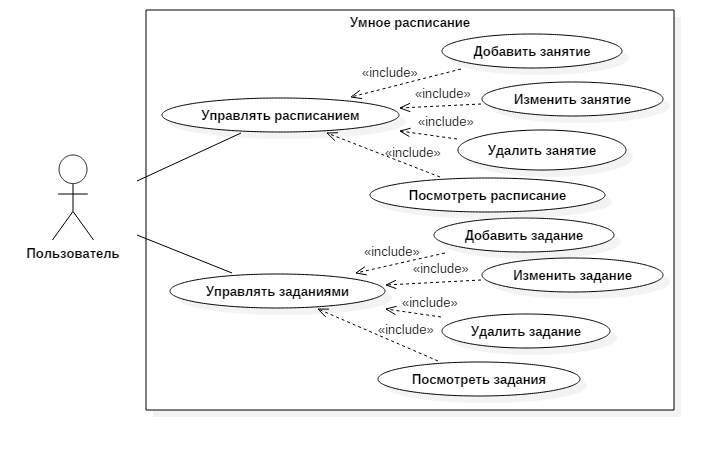
\includegraphics[scale=0.7]{pics/usecase}
		\caption{Диаграмма прецедентов использования} 
		\label{pic:use_case_diagram} % название для ссылок внутри кода
	\end{center}
\end{figure}

Выше на рис. \ref{pic:use_case_diagram} показана диаграмма прецедентов использования умного расписания. Пользователь может работать с расписанием: добавлять, изменять и удалять занятия, а также работать с заданиями: добавлять, изменять и удалять задания.

\subsection{Выводы}

В данном разделе было определены требования к приложению \textit{Smart Schedule}, его концепция, диаграмма прецедентов использования приложения и минимально работоспособный продукт.

\section{Проектирование приложения Smart Schedule}

В процессе проектирования было решено выделить 3 подпроекта:
\begin{enumerate}
\item \textbf{mongo} -- модуль, содержащий логику работы с базой данных и предоставляющий интерфейс \texttt{Database API};
\item \textbf{core} -- библиотека, содержащая бизнес-логику приложения и предоставляющая интерфейс \texttt{Core API};
\item \textbf{rest} -- RESTful\footnote{https://ru.wikipedia.org/wiki/REST} веб-сервис, предоставляющий интерфейс \texttt{REST API};
\item \textbf{android} -- клиентское приложение для ОС Android.
\end{enumerate}

\subsection{Диаграмма компонентов}

\begin{figure}[H]
	\begin{center}
		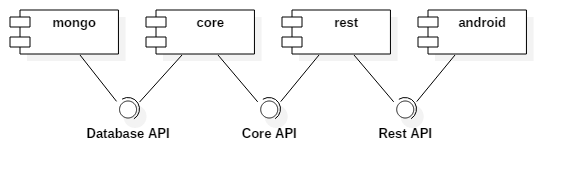
\includegraphics[scale=0.7]{pics/components}
		\caption{Диаграмма компонентов} 
		\label{pic:component_diagram}
	\end{center}
\end{figure}

Выше на рис. \ref{pic:component_diagram} представлена диаграмма компонентов, где \textbf{mongo} -- база данных; \textbf{core} -- библиотека; \textbf{rest} -- веб-сервис и \textbf{android} -- Android приложение.

\subsection{Интерфейс библиотеки}

\subsection{Хранение данных}

\subsection{Выводы}

В данной главе было рассмотрено проектирование умного расписания: деление на подпроекты \texttt{mongo}, \texttt{core}, \texttt{rest} и \texttt{android}, определение диаграммы компонентов, выделение основных методов интерфейса, а также принятно решение об использовании базы данных \texttt{Mongo DB}.

\section{Реализация приложение Smart Schedule}

\subsection{Среда разработки}

В процессе разработки использовалась интегрированная среда разработки \texttt{IntelliJ IDEA 2016 3.1} от компании \texttt{JetBrains}. Для сборки проекта использовалась система автоматической сборки \texttt{Gradle 3.1}. Был выбран уровень языка Java \texttt{1.8}.

\subsection{Реализация библиотеки}

\subsection{Реализация хранения данных}

\subsection{Реализация веб-сервиса}

\subsection{Реализация Andorid приложения} 

\subsection{Снимки экранов пользовательского интерфейса}

\subsection{Выводы}

В данной главе была рассмотрена реализация приложения Smart Schedule, рассмотрены основные классы библиотеки, рассмотрена реализация модулей, а также приведены снимки экрана работающего приложения.

\section{Процесс обеспечения качества и тестирование}

\subsection{Утилиты и плагины}

\subsection{Непрерывная интеграция}

\subsection{Просмотр кода и демонстрации}

\subsection{Тестирование}

\subsection{Выводы}

В данной главе были рассмотрены используемые в процессе разработки утилиты и плагины для среды разработки \texttt{IntelliJ IDEA}, оценен вклад просмотра кода и демонстраций, оценена полезность практики непрерывной интеграции, а также сделаны выводы о тестировании приложения.

\section{Выводы}

При выполнении задания были закреплены навыки в работе с объектно-ориентированным программированием, получен опыт в организации и разработке проекта на языке \texttt{Java}, создании и автоматизации модульных тестов, а также в использовании утилит и плагинов для интегрированной среды разработки, помогающих в разработке приложений.

Результатом работы стало приложение на Java, которое позволяет вводить и просматривать учебное расписание и домашние задания, необходимые выполнить к определенной дате.

\end{document}